\pdfoutput=1
\pdfminorversion=7
\documentclass[11pt,a4paper]{article}
\usepackage[T1]{fontenc}
\usepackage[utf8]{inputenc}
\usepackage{lmodern}
\usepackage[a4paper,margin=2.25cm]{geometry}
\usepackage{microtype,parskip}
\usepackage{amsmath,amssymb,amsthm}
\usepackage{graphicx,booktabs,tabularx,array}
\usepackage[font=small,labelfont=bf]{caption}
\usepackage[round,authoryear]{natbib}
\usepackage{xcolor}
\usepackage[colorlinks=true,linkcolor=black,citecolor=black,urlcolor=blue!45!black]{hyperref}
\hypersetup{pdftitle={From Governance Reviews to Task Substitution: DGF-Bench and the Role of Forward Deployed Engineers},pdfauthor={Jeremy Canale},pdfsubject={Synthetic governance review evaluation and a field-validation agenda}}
\newcolumntype{L}{>{\raggedright\arraybackslash}X}
\newcolumntype{P}[1]{>{\raggedright\arraybackslash}p{#1}}
\newtheorem{proposition}{Proposition}
\makeatletter
\newcommand{\rowsinput}[1]{\@@input #1.tex }
\makeatother
\setlength{\emergencystretch}{2em}
\title{\textbf{From Governance Reviews to Task Substitution}\\[0.4em]
\large DGF-Bench and the Role of Forward Deployed Engineers}
\author{Jeremy Canale\\\normalsize\texttt{contact@jeremycanale.com}\\
\normalsize\url{https://www.jeremycanale.com}}
\date{September 2026}
\begin{document}
\maketitle
\begin{abstract}
Enterprise governance reviews transform project evidence into decisions, conditions, and actions.
We evaluate whether tool-using language models can perform this work under explicit policies,
using DGF-Bench: 300 synthetic Buy, Integrate, and Build projects with generated documents,
architectures, simulated records, and sequential review gates. Agents have access to authoritative
structured facts as well as documents. Across 899 evaluable model--project runs, Gemini 3.8 Flash,
GPT-5.6 Luna, and DeepSeek v4.1 Flash achieve strict gate success of 94.98\%, 83.29\%, and
74.18\%, respectively. Complete-route success is 76.92\%, 42.33\%, and 24.67\%; recorded
API cost totals USD~87.02. Gemini has 100\% disposition accuracy: all its strict failures concern
evidence conformity. We therefore distinguish decision quality from lexical traceability instead
of interpreting the gate--route gap as a general reasoning failure. These results support the
technical prospect of automating the represented review tasks. We formulate a conditional
task-substitution hypothesis and specify how forward deployed engineers could connect review
automation to operational evidence, authority, exception handling, and measurement of human work.
A compact labor account shows why benchmark accuracy is not a staffing-reduction estimate.
Independent human comparison, semantic evidence adjudication, scaffold-removal tests, and a
prospective enterprise cohort are specified as follow-up studies, not completed experiments.
The hypothesis of 80\% fewer required DGF FTE by 2033 is retained as a field-testable projection
with an explicit historical-baseline requirement. All benchmark sources, traces, and datasets
are public. This manuscript reorganizes an existing experiment; it reports no new model trials.
\end{abstract}
\noindent\textbf{Keywords:} governance reviews; AI agents; forward deployed engineering; benchmark; task substitution; human workload.

\section{Introduction: replacing execution, preserving the function}

Before an enterprise buys software, connects systems, or releases an application, people review
its architecture, security, contracts, cost, and operational readiness. The required outputs are
decisions and their supporting work: identify a missing agreement, reject an unsafe network
design, require a recovery test, or authorize a conditional release. These functions persist
even if software performs work previously assigned to analysts, architects, and committee
support staff. A professional title is an organizational allocation of tasks, not a technical
specification of how those tasks must be executed.

This paper argues that a Digital Governance Framework (DGF), understood as an enterprise's
connected review gates, is a tractable candidate for early substitution of human review tasks
by agentic systems. The claim concerns execution: an agent that produces a draft for someone
to redo has supplied assistance; a system that completes an accepted review has performed that
task. A workflow can contain substituted tasks and remaining human decisions at the same time.
The relevant system can combine language models, deterministic software, and escalation.
Replacing every rule check with a language-model call is neither necessary nor desirable.

Figure~\ref{fig:dgf-routes} makes this organization concrete: the same project dossier moves
through several specialist reviews, each producing a decision and its supporting record.
Buying a solution, connecting systems, and building an application require different review
sequences. General consolidates the preceding reviews into the route's governance record.

\begin{figure}[!htb]
\centering
\begin{tikzpicture}[
  x=2.5cm,y=1cm,
  gate/.style={draw=black!55,rounded corners=2pt,minimum height=0.64cm,
    text width=2.08cm,align=center,inner sep=2pt,font=\small},
  consolidate/.style={gate,fill=black!8,draw=black!75},
  flow/.style={-{Stealth[length=1.5mm]},draw=black!65,semithick},
  route/.style={anchor=west,font=\small}
]
\node[route] at (-0.46,0.62) {\textbf{BUY} \quad Purchase a solution};
\node[gate,fill=blue!5] (b1) at (0,0) {Procurement};
\node[gate,fill=blue!5] (b2) at (1,0) {Legal};
\node[gate,fill=blue!5] (b3) at (2,0) {Compliance};
\node[gate,fill=blue!5] (b4) at (3,0) {Security};
\node[gate,fill=blue!5] (b5) at (4,0) {IT};
\node[consolidate] (b6) at (5,0) {General};
\foreach \a/\b in {b1/b2,b2/b3,b3/b4,b4/b5,b5/b6}
  \draw[flow] (\a) -- (\b);

\node[route] at (-0.46,-0.73) {\textbf{INTEGRATE} \quad Connect existing systems};
\node[gate,fill=teal!6] (i1) at (0,-1.35) {IT};
\node[gate,fill=teal!6] (i2) at (1,-1.35) {Architecture};
\node[gate,fill=teal!6] (i3) at (2,-1.35) {Security};
\node[gate,fill=teal!6] (i4) at (3,-1.35) {Legal};
\node[gate,fill=teal!6] (i5) at (4,-1.35) {Compliance};
\node[consolidate] (i6) at (5,-1.35) {General};
\foreach \a/\b in {i1/i2,i2/i3,i3/i4,i4/i5,i5/i6}
  \draw[flow] (\a) -- (\b);

\node[route] at (-0.46,-2.08) {\textbf{BUILD} \quad Develop an application};
\node[gate,fill=orange!7] (d1) at (0,-2.7) {IT};
\node[gate,fill=orange!7] (d2) at (1.25,-2.7) {Architecture};
\node[gate,fill=orange!7] (d3) at (2.5,-2.7) {Security};
\node[gate,fill=orange!7] (d4) at (3.75,-2.7) {Tech\\Readiness};
\node[consolidate] (d5) at (5,-2.7) {General};
\foreach \a/\b in {d1/d2,d2/d3,d3/d4,d4/d5}
  \draw[flow] (\a) -- (\b);

\node[font=\small,align=center] at (2.5,-3.48)
  {\textbf{At each gate:} inspect the dossier; record findings, evidence, actions, and a decision.};
\end{tikzpicture}
\caption{Three DGF workflows evaluated in DGF-Bench. A project follows the route matching its
need. Arrows show review order and information handoffs; General consolidates preceding reviews.
The benchmark runs all scheduled gates, including after a refusal. These are example governance
routes, not automatic approvals or a universal enterprise standard.}
\label{fig:dgf-routes}
\end{figure}


The DGF is attractive because it already organizes work into dossiers, policies, named
authorities, bounded decisions, and recorded handoffs. This gives engineering a starting point
that open-ended management lacks. The same features also reveal why a fluent agent is insufficient:
facts may be missing, exceptions expensive, evidence unfaithful, and commitments unauthorized.
Our claim is that these are explicit conditions of substitution, rather than reasons to assume
that the current human task allocation must remain permanent. Whether DGF is earlier or easier
to automate than every other business function is a comparative hypothesis, not an observed ranking.

We connect three contributions. First, a gate-contract formulation identifies information,
validity, and authority requirements for delegating review execution. A source counterexample
shows when no reviewer can satisfy a fixed decision contract from the permitted information.
Second, a complete labor account gives a substitution threshold: reducing routine execution
only reduces required human work if exception handling, verification, correction, and support
remain below a computable budget. Third, DGF-Bench provides a public, controlled measurement
of specified review tasks and their failure modes, including a deterministic control and
repeated trajectories. The purpose of linking them is to make the route from an agent score
to a workforce claim inspectable; none of the three substitutes for the others.

\subsection{Research questions and units of analysis}

We organize the argument around three questions with different observational units.
\emph{First, can software execute a specified gate contract?} Its unit is a review occurrence,
with fixed inputs, rules, and acceptance conditions. DGF-Bench measures this question in a
synthetic environment. \emph{Second, can that execution remain dependable across a project?}
Its unit is the complete route, including the evidence and conditions passed between gates.
Route success and repeated trajectories address parts of this question. \emph{Third, does
deployment reduce the human work required to deliver the governed output?} Its unit is an
operating population over a stated period. Answering it requires a labor account, including
work added outside the nominal review team. This third quantity is not present in an API trace.

The units cannot be exchanged without assumptions. Five thousand scored gates are not five
thousand independent companies. A successful run on a generated dossier is not a measured
number of hours saved. A refusal may be a successful review even though the underlying project
does not proceed. Defining these distinctions makes a positive replacement claim more precise:
software can execute an accepted task while humans remain responsible for setting its scope,
maintaining its infrastructure, or resolving a subset of exceptions.

\begin{table}[!htb]
\centering\small
\caption{Claim structure and evidence required. A result at one level does not supply the
missing observation at another.}
\label{tab:claim-structure}
\begin{tabularx}{\linewidth}{@{}P{2.8cm}LL@{}}
\toprule
Claim & Observable test & Evidence in this paper\\
\midrule
Contract execution & Decision, findings, actions, evidence, and mandate meet fixed criteria & Original runs and deterministic control\\
Workflow reliability & Every required gate succeeds; repeated trajectories remain successful & Complete-route scores and 135 additional runs\\
Net task substitution & Accepted output requires fewer total human hours & Accounting conditions and illustrative calculations\\
Ecosystem workforce reduction & Comparable governed output and quality with a lower complete FTE account & Dated hypothesis and a measurement protocol\\
\bottomrule
\end{tabularx}
\end{table}

The central thesis is consequently about the implementation of a function. Organizations may
still require architecture assurance, a security judgment, or evidence of operational readiness.
That continuing requirement does not establish that every dossier needs the same manual
execution. At the same time, describing a function as a contract does not make its evidence
available or resolve policy disagreement. The proposed engineering work is to turn the subset
with adequate information and delegated authority into executable review services, and then
measure the cost of the boundary that remains.

The paper proceeds from the contract to the labor account, then to its FDE implementation and
experimental evidence. We conclude with a deployment test for the workforce hypothesis.
This manuscript synthesizes the longer \emph{The Last Human Gate} and replaces the previous
empirical companion in the repository. The versions share their experimental record;
the expanded exposition reports no additional model calls or enterprise observations.

\section{Evidence: executing governance contracts}
\label{sec:benchmark}

\paragraph{Design and scope.}
DGF-Bench tests the execution of a specified review task: inspect permitted evidence, choose a
disposition, identify findings and required actions, cite the supporting observations, and respect
the authorization contract. A seeded generator constructs 300 fictional projects, 100 each on
Buy, Integrate, and Build routes. Buy follows Procurement, Legal, Compliance, Security, IT, and
General; Integrate follows IT, Architecture, Security, Legal, Compliance, and General; Build
follows IT, Architecture, Security, Tech Readiness, and General. This gives 1,700 gate occurrences
per model. The dossiers include project charters and review requests, architecture diagrams,
technical designs, supplier and legal records, and operational test evidence. Decision-coverage
sampling balances applicable outcomes. Difficulty setting 4 controls generator parameters;
it is not a validated scale of reasoning difficulty. The 300 projects have distinct architecture
and complete decision-fact signatures, although some gate-level patterns recur.

The tested information condition supplies both executable policies and an authoritative
structured \texttt{REVIEW\_FACTS} snapshot. Models can read allowed evidence and use simulated
enterprise tools; evaluator-only reference files are inaccessible. The model is the reviewer,
not the generator of the project. Every gate returns one of \texttt{GO},
\texttt{GO\_WITH\_RESERVATIONS}, \texttt{REWORK}, \texttt{SUSPENSION}, or \texttt{NO\_GO}.
Correctly refusing a deficient proposal counts as success. Later gates receive the model's actual
upstream reviews, and General consolidates the route.

Three exact OpenRouter endpoint identifiers were evaluated on 22--23 September 2026:
\nolinkurl{google/gemini-3.8-flash}, \nolinkurl{openai/gpt-5.6-luna}, and
\nolinkurl{deepseek/deepseek-v4.1-flash}. Temperature was zero, vision was \texttt{auto},
and each gate permitted at most 20 turns, 40 tool calls, and 8,192 output tokens per turn.
Of 900 planned model--project runs, 899 and their 5,094 gates are evaluable. One Gemini
Integrate run failed at its first gate because of a provider generation error; its six gates
are excluded. Recorded failed attempts remain in the cost accounting and released traces.

\paragraph{Outcomes and comparison.}
The frozen deterministic evaluator requires a correct disposition, exact finding and action
sets, observed evidence references and exact observed field/value excerpts, and the correct authorization
indicator. A \emph{strict gate success} passes every component; a \emph{complete route} passes
every gate. Disposition accuracy alone therefore does not measure a complete review. Validated
conditional approvals can change the effective reference outcome. A false approval proceeds
when that effective reference requires rework, suspension, or refusal; a critical miss omits
a finding classified as critical by the policy.

A deterministic control reads the same public snapshots and executes the public policy functions,
then writes its predictions before a separate process invokes the frozen scorer. It does not
read hidden references during generation, request optional conditional approvals, or extract
facts from documents. It can quote full snapshots without the models' per-turn output-token
limit. Its perfect score establishes that the formalized review kernel is software-executable;
this condition establishes no incremental benefit from language-model inference.

\begin{table}[!htb]
\centering\small
\caption{Task execution on the original population and repeated trajectories. Counts preserve
the original strict endpoint. Sensitivity accepts specified structural evidence matches;
it is post-hoc and is not a semantic adjudication. The deterministic control was not repeated.}
\label{tab:compact-evidence}
\setlength{\tabcolsep}{4pt}
\begin{tabularx}{\linewidth}{@{}Lrrrr@{}}
\toprule
Outcome & Gemini & Luna & DeepSeek & Rules\\
\midrule
Evaluable projects & 299 & 300 & 300 & 300\\
Evaluable gates & 1,694 & 1,700 & 1,700 & 1,700\\
Correct dispositions & 1,694 & 1,668 & 1,619 & 1,700\\
Strict gate successes & 1,609 & 1,416 & 1,261 & 1,700\\
Strict gate success (\%) & 94.98 & 83.29 & 74.18 & 100.00\\
Complete routes & 230 & 127 & 74 & 300\\
Complete routes (\%) & 76.92 & 42.33 & 24.67 & 100.00\\
Evidence-only failures & 85 & 221 & 338 & 0\\
False approvals / critical misses & 0 / 0 & 1 / 3 & 1 / 1 & 0 / 0\\
Sensitivity: successful gates & 1,678 & 1,454 & 1,313 & ---\\
Sensitivity: complete routes & 284 & 144 & 85 & ---\\
\midrule
\multicolumn{5}{@{}l}{\emph{Follow-up: 15 existing dossiers, three trajectories per model}}\\
Strict gates / 255 & 245 & 211 & 187 & ---\\
Complete routes / 45 & 35 & 19 & 11 & ---\\
Dossiers passing all three / 15 & 9 & 3 & 0 & ---\\
\bottomrule
\end{tabularx}
\end{table}

\paragraph{What succeeds, and what still fails.}
Gemini reaches the correct effective disposition on every evaluable gate and satisfies all
non-evidence components; its 85 strict failures concern evidence conformity. Its strict gate
rate is 94.98\% (95\% interval 93.86--96.04), but only 76.92\% of complete routes pass
(71.82--81.34). Luna and DeepSeek also exhibit a large gate--route gap, alongside substantive
errors: Luna approves one Legal review despite a missing data-processing agreement, and
DeepSeek submits a placeholder \texttt{GO} at forced finalization when address overlap
requires \texttt{NO\_GO}. The model comparison therefore distinguishes successful disposition,
complete documented review, and dependable execution of a whole route.

Gate intervals resample whole cases within routes (2,000 draws, seed 81931); route intervals
use Wilson bounds. They describe the generated population, retaining within-project dependence.
They do not treat 5,094 gates as independent organizations. The common 299-case comparison
preserves the ranking; its paired intervals and complete component tables are released.

An audit of all 690 gates with a failed evidence component leaves the primary scores unchanged
and applies one declared sensitivity rule: accept exact relevant field/value subsets from one
observed object despite field order or equivalent numeric serialization. No quote is repaired,
no tool observation invented, and no join across different objects promoted. This recovers
69 Gemini, 38 Luna, and 52 DeepSeek gates (Table~\ref{tab:compact-evidence}). Gemini's rate
becomes 99.06\% at gate level and 94.98\% at route level. The interpretation is specific:
much of this model's measured route failure depends on the evidence representation contract.
The audit does not establish full premise coverage or independently validated semantic support.

\paragraph{A concrete delegated review.}
In \nolinkurl{DGF-BLD-035200_build}, a generated vendor-portal project, Gemini's Tech Readiness
review finds a draft runbook. It names \texttt{TR-OPS-001}, proposes
\texttt{COMPLETE\_OPERATIONAL\_HANDOVER}, and cites the observed value
\texttt{"runbook\_status": "draft"}. After consulting an active mandate, it invokes the
conditional-approval tool with a requirement to approve the runbook before production cutover.
The tool executes the authorization but explicitly leaves the finding unresolved. The model
submits \texttt{GO\_WITH\_RESERVATIONS} with the finding and action retained, satisfying the
strict contract. This post-hoc example demonstrates a performed review and authorized workflow
transition, not completed remediation. Authority resides in the surrounding system: across the
original experiment, Gemini makes 466 rejected conditional-approval calls as well as 398
executed approvals. Its absence of scored false final approvals cannot be attributed solely
to consistently correct initial action selection.

\paragraph{Repeatability and the remaining boundary.}
The follow-up fixes 15 existing dossiers, five per route, before collecting three new
trajectories for every model--dossier pair: 135 completed runs and 765 gates. No best-of-three
selection is used. Gemini, Luna, and DeepSeek pass respectively 35, 19, and 11 of 45 routes;
only nine, three, and zero dossiers pass on all three trajectories. All follow-up false-approval
and critical-miss counts are zero. Provider routing is not fixed, so these observations measure
repeatability of the recorded system rather than intrinsic model randomness. Original and
follow-up recorded API costs are USD~87.015829172 and USD~12.5598870228, totaling USD~99.58;
development, local computation, human review, and deployment are not costed.

The information counterexample in Section~\ref{sec:contract} identifies a different failure
boundary: some proposed document-only inputs cannot determine the required decision. Together,
the observed executions and the source check show both an automatable formalized task and
a specific obstruction that must be resolved before extending its scope.

\section{What the scores establish}
\label{sec:measurement}

\subsection{A near-saturated disposition task and a stricter trace contract}

Gemini's 100\% disposition accuracy is a strong result under the declared conditions. It also
indicates that this sample offers little remaining discrimination on that component for this
endpoint. The model can read explicit rules and authoritative structured facts; this experiment
does not isolate how much ability is needed to recover those facts from documents. The deterministic control now executed on the same 300 dossiers reaches full strict success.
It demonstrates that the supplied executable rules and structured facts are sufficient to solve
this instance of the task without model inference. Model success remains an observation about
model-based execution, but does not establish an incremental benefit over direct rule execution.

Strict success answers a different question: does the entire submitted review satisfy the
implemented contract, including exact evidence provenance? It is useful when downstream processing
requires precise traceability, but it is not a direct measure of independent expert judgment.
The selected Architecture example shows a correct decision and correct values with a failed
excerpt because two fields were reversed. The Legal false approval by Luna and DeepSeek's
placeholder approval illustrate materially different errors. Those classes should not be
collapsed into a single narrative about reasoning failure.

\begin{table}[!htb]
\centering\small
\caption{Separate observed outcomes. Evidence-only failures have no other failing scored component;
they are not all established to be harmless formatting errors.}
\begin{tabularx}{\linewidth}{@{}Lrrrr@{}}
\toprule
Outcome & DeepSeek & Gemini & Luna & Rules\\
\midrule
Correct dispositions / evaluable gates & 1,619/1,700 & 1,694/1,694 & 1,668/1,700 & 1,700/1,700\\
Strictly successful gates & 1,261 & 1,609 & 1,416 & 1,700\\
Evidence-only gate failures & 338 & 85 & 221 & 0\\
Other strict gate failures & 101 & 0 & 63 & 0\\
False approvals & 1 & 0 & 1 & 0\\
Critical finding misses & 1 & 0 & 3 & 0\\
\bottomrule
\end{tabularx}
\end{table}

The strict gate--route gap for Gemini is consequently a compounding of evidence-conformity
failures across routes, not evidence of incorrect final dispositions. A strict route fails
when any component at any gate fails. This is the intended operational definition, but the
figure 76.92\% must be read with that definition. We retain both the original scoring rule and
the component breakdown. A declared post-hoc sensitivity analysis can quantify representation effects, but cannot
replace the primary score or imply that every lexical failure is a dangerous decision.

\subsection{Executed deterministic control}
\label{sec:rules-control}

A separate generation process reads each dossier's public route and gate contract. For each
occurrence it reads the authoritative snapshot through the same public evidence reader, executes
\texttt{rule\_definition\_python} from the supplied policy, combines finding dispositions using
the declared priority order, and sets the authorization indicator using the declared disposition
list. Finding construction and result aggregation are implemented from that public interface.
The policy functions are the executable definitions supplied to the language models; they are
not a separately learned policy or an independently validated governance standard.

The comparator retains the base disposition and never requests optional conditional risk
acceptance, a strategy explicitly permitted by the policy. It cites complete observed JSON
snapshots as exact evidence excerpts and propagates its own earlier decisions to General.
This exploits the absence of a quote-length cap; the program is not subject to the models'
per-turn output-token limit. It does not attempt document extraction or
image interpretation. A read guard blocks evaluator-only reference files during generation,
and the generation process asserts that neither the evaluator nor scorer module was imported.
All predictions and observation records are written before a second process invokes the frozen
scorer, which is allowed to read the hidden references for evaluation.

The result is \textbf{1,700/1,700 strict gate successes and 300/300 complete routes}, with no
false approvals or critical misses. Model API expenditure is zero; programming and local
compute are not costed. On the 299 cases shared with Gemini, the control also succeeds on all
1,694 gates. Optional approval choices can differ between systems, and each is scored against
the protocol's effective reference; full conformity does not mean identical submitted decisions.

This is a scaffold-sufficiency control. It does not validate the business rules independently,
because the public policy and evaluator share their definitions. It does show that an LLM is
unnecessary for achieving the measured endpoint when those functions and structured facts are
already available. The main unresolved model contribution therefore lies in tasks that this
run did not isolate: recovering facts, resolving ambiguity, and interacting with less structured
operational evidence. Claims about such a contribution require the proposed ablations and
external validation, rather than a higher score on this saturated contract.

\subsection{Executed structural audit of Gemini's 85 failures}
\label{sec:structural-audit}

We inspected every Gemini strict-failure gate against its saved submission and pre-submission
read events. The 85 failed gates contain 84 flagged finding-support items: a gate may contain
several items, while a citation-only failure may contain none. The audit parses each quote as
a JSON object fragment, rejects duplicate keys, and checks all quoted field values against a
single observed object while ignoring key order and numeric serialization such as 30 versus
30.0. Booleans remain distinct from numbers; 10 cannot match 100. A second diagnostic records
where values exist across different objects, without treating a flattened join as a faithful
single-object excerpt. This is a post-hoc structural test, not independent expert adjudication.

\begin{table}[!htb]
\centering\small
\caption{Exhaustive post-hoc audit of Gemini strict failures. Categories describe recorded
representation and observation defects, not new semantic pass rates.}
\begin{tabularx}{\linewidth}{@{}LrL@{}}
\toprule
Gate category & Gates & Item-level explanation\\
\midrule
All flagged quotes match observed objects after structural normalization & 69 & 75 flagged finding items preserve the checked field values within an observed object.\\
Flattened cross-object excerpts & 9 & 9 flagged items combine observed values from separate objects; paths are retained for inspection.\\
Required evidence-tool observation absent & 7 & All cite \texttt{UPSTREAM\_DECISIONS} without the corresponding read event.\\
\bottomrule
\end{tabularx}
\end{table}

For example, a flattened high-availability excerpt combines business criticality from the
project object with redundancy flags from the architecture-profile object. Those values are
present, but the quoted combined object was not observed. In the seven citation cases, upstream
reviews were also included in the gate prompt; the defect is the missing required evidence-tool
read, not proof that the model never received the underlying information. Neither a corrected
quote nor an invented read event is inserted into the original trace.

The audit identifies representation-related causes for the 78 excerpt-failure gates and a
separate observation-contract cause for seven gates. It supplies no independent judgment that
every policy inference is justified or that every necessary premise was cited. The single-object
matching check accepts relevant field values rather than proving full entailment, as does the
original lexical checker. We retain the original 94.98\% strict gate and 76.92\% strict route
rates and report the audit alongside them. No revised whole-benchmark semantic rate is claimed.
Complete excerpts, observed contents, matched paths, categories, and source trace identifiers
are released with the audit script.

\subsection{All-model structural sensitivity and procurement failures}
\label{sec:all-model-audit}

We apply the same post-hoc check to every original gate with evidence fidelity below one:
354 DeepSeek, 85 Gemini, and 251 Luna gates. A gate passes the relaxed endpoint if it originally
passed strictly, or if all unchanged non-evidence components pass, its required citations were
observed, and each originally unsupported finding has a relevant exact field/value subset
within one observed object. Cross-object joins are not promoted. Quotes and read events are
not repaired. Original lexical successes remain accepted, so this is a lexical-or-structural
sensitivity endpoint, not a replacement semantic metric. A matching relevant field need not
supply every premise of a finding.

\begin{table}[!htb]
\centering\small
\caption{Original strict versus post-hoc lexical-or-structural success on the same saved
trajectories. Relaxation changes the evidence criterion only; it is not a new model result.}
\begin{tabular}{@{}lrrrr@{}}
\toprule
& \multicolumn{2}{c}{Gates} & \multicolumn{2}{c}{Complete routes}\\
Model & Strict & Relaxed & Strict & Relaxed\\
\midrule
Gemini & 1,609/1,694 & 1,678/1,694 & 230/299 & 284/299\\
Luna & 1,416/1,700 & 1,454/1,700 & 127/300 & 144/300\\
DeepSeek & 1,261/1,700 & 1,313/1,700 & 74/300 & 85/300\\
\bottomrule
\end{tabular}
\end{table}

Gate success rises from 94.98\% to 99.06\% for Gemini, 83.29\% to 85.53\% for Luna, and
74.18\% to 77.24\% for DeepSeek. Complete-route success rises to 94.98\%, 48.00\%, and
28.33\%, respectively. The large Gemini gate--route gap is therefore highly sensitive to
serialization. The smaller changes for the other endpoints show that this explanation does
not transfer uniformly across models.

\begin{table}[!htb]
\centering\small
\caption{Classification of evidence-only failed gates. ``Unresolved'' means not accepted by
this structural parser, not a demonstrated false claim. Categories are mutually exclusive.}
\begin{tabularx}{\linewidth}{@{}Lrrr@{}}
\toprule
Category & DeepSeek & Gemini & Luna\\
\midrule
Same-object matches for all failed finding items & 52 & 69 & 38\\
Cross-object excerpt remains & 2 & 9 & 46\\
Citation/observation defect & 109 & 7 & 1\\
Unresolved structural or support defect & 175 & 0 & 136\\
\midrule
Total evidence-only failures & 338 & 85 & 221\\
\bottomrule
\end{tabularx}
\end{table}

Procurement localizes an especially important contrast. There are 100 evaluable Procurement
gates per model. Gemini makes 100 correct decisions and passes 96 strictly; all four failures
are budget-related cross-object excerpts. DeepSeek makes 97 correct decisions but passes only
43 strictly, with 54 evidence-only failures. Luna makes 96 correct decisions but passes 33
strictly, with 63 evidence-only failures. Structural relaxation recovers no additional DeepSeek
Procurement gate and only one Luna gate. Many failed items are not parseable as object fragments;
others combine separate objects or lack valid support. These categories require semantic review
before being called hallucinations. Procurement is thus mainly an evidence-contract bottleneck
in this sample, despite some substantive decision errors. Per-rule classifications and original
quotes are included in the released item-level audit.

Independent semantic adjudication remains unperformed. A suitable rubric would separately
label observed access, source/span fidelity, factual entailment, and sufficiency for the policy
finding; two masked domain-qualified adjudicators would label independently and resolve disputes
under a fixed procedure. Both failures and a probability sample of passes should be assessed.
A full semantic route rate requires adjudicating all required support on the routes counted,
not just forgiving selected failed quotes.

\subsection{Decision confusion and the effective reference}

The full confusion matrices in Appendix~A show 81 incorrect DeepSeek dispositions and 32
incorrect Luna dispositions; Gemini has none under the effective-reference score. DeepSeek's
errors are mostly more restrictive than the reference under the policy's priority order
(76/81), including 35 GO-to-REWORK and 23 GO\_WITH\_RESERVATIONS-to-REWORK outcomes. Luna has
10 more-restrictive and 22 less-restrictive errors, including 17 SUSPENSION-to-REWORK outcomes.
A less-restrictive error between blocking decisions is not automatically a false approval;
each of these two models has one scored false approval.

The effective reference incorporates verified conditional approvals and their authorized
upstream consequences. It is not always the initial label. Agreement with the unmodified base
reference is 1,553/1,700 for DeepSeek, 1,553/1,694 for Gemini, and 1,568/1,700 for Luna, versus
1,619/1,700, 1,694/1,694, and 1,668/1,700 with the effective reference. Gemini's 141 base-label
differences comprise 139 local conditional approvals and two General outcomes reflecting
upstream authorized changes. The evaluator checks mandate and approval conditions; the model
cannot make a decision correct merely by declaring it approved. Reporting both agreements
clarifies the target: the primary metric measures conformity after allowed actions, while
initial-label agreement measures a different, action-insensitive target.

\subsection{Executed repeated trajectories on 15 dossiers}
\label{sec:repetitions}

Before launching follow-up calls, we selected five dossiers without replacement per route
from sorted identifiers with Python \texttt{random.Random(23092026)}. Selection did not use
model outcomes. The local plan fixed three new trajectories per model--case pair, giving
15 dossiers, three endpoints, 135 runs, and 765 gates. This is a local analysis plan, not an
external preregistration. The original historical trajectories are not counted as a fourth
exchangeable repeat and are not pooled into the follow-up rates.

Collection on 23--24 September 2026 used byte-verified copies of the existing dossiers and the
frozen benchmark source. All three repetitions have identical recorded protocol identities:
temperature zero, agent handoffs, automatic vision, 20 turns, 40 tool calls, and 8,192 output
tokens per turn. There were three workers, one per model. Each repeat had a separate output
directory. Infrastructure recovery retained completed gate prefixes within that trajectory;
successful completed routes were not rerun or selected on their score.

All 135 final runs are evaluable and all 765 gates attempted. Retained error checkpoints
record 46 key-limit refusals and two provider-finish errors. Two Gemini runs resumed seven
completed gates in total. One truncated response is recorded for Gemini and no resolved-model
mismatches are recorded. The total USD~12.5598870228 includes unsuccessful paid attempts;
all ledger entries have known costs. The authorization was increased from USD~20 to USD~50
after a separate API-key limit interrupted collection. This did not change the case sample,
repeat count, or inference settings.

\begin{table}[!htb]
\centering\small
\caption{Three fresh trajectories on the same 15 dossiers. Strict gate counts are out of 85
per repeat; complete-route counts are out of 15. The last column requires all gates to pass
on all three trajectories of a dossier.}
\label{tab:repetitions}
\begin{tabular}{@{}lrrrrrrr@{}}
\toprule
& \multicolumn{3}{c}{Strict gates / 85} & \multicolumn{3}{c}{Complete routes / 15} & All three\\
Model & R1 & R2 & R3 & R1 & R2 & R3 & / 15\\
\midrule
Gemini & 82 & 82 & 81 & 12 & 12 & 11 & 9\\
Luna & 73 & 71 & 67 & 8 & 7 & 4 & 3\\
DeepSeek & 63 & 64 & 60 & 3 & 4 & 4 & 0\\
\bottomrule
\end{tabular}
\end{table}

\begin{table}[!htb]
\centering\small
\caption{Follow-up rates pooled over three trajectories, with exploratory 95\% case-cluster
bootstrap intervals in brackets. Every model has 255 scored gates and 45 completed runs.}
\begin{tabular}{@{}lrrr@{}}
\toprule
Model & Strict gate success & Complete-route success & API cost (USD)\\
\midrule
Gemini & 96.08\% [93.33, 98.43] & 77.78\% [62.22, 91.11] & 10.3889\\
Luna & 82.75\% [75.29, 89.80] & 42.22\% [22.22, 62.22] & 0.7499\\
DeepSeek & 73.33\% [66.67, 79.61] & 24.44\% [13.33, 37.78] & 1.4212\\
\bottomrule
\end{tabular}
\end{table}

The bootstrap uses 10,000 draws, seed 24092026, resampling five entire dossiers within each
route with replacement. Each sampled dossier retains all its gates and all three trajectories.
Percentile endpoints use linear interpolation. These intervals reflect only this small,
stratified synthetic sample, not 255 independent observations or uncertainty over enterprises.
In particular, zero observed all-three successes for DeepSeek is not proof of zero population
success probability; its degenerate empirical bootstrap interval is not a useful risk bound.

Gemini has 255/255 correct dispositions, Luna 246/255, and DeepSeek 245/255. There are zero
scored false approvals and critical misses for each model in this follow-up. Evidence fidelity
fails on 10, 36, and 59 gates, respectively. These are new strict scores; the structural audit
of the original 85 Gemini failures is not silently applied to these new traces.

The ranking persists in each repetition, but a similar overall rate does not imply repeatable
success on every dossier. Complete-route pass/fail changes across repeats for five Gemini,
six Luna, and eight DeepSeek dossiers. Only nine, three, and zero dossiers, respectively,
pass all three times. Exact gate dispositions remain identical across repeats on all 15 Gemini
dossiers, ten Luna dossiers, and six DeepSeek dossiers. Optional authorized conditional approvals
can legitimately change a disposition, so disagreement is not by itself an error.

Provider routing was not fixed: DeepSeek records eight providers, Gemini Google AI Studio,
and Luna OpenAI. Consequently, variability cannot be attributed solely to intrinsic model
randomness. Temperature zero, small sample size, existing generated cases, and infrastructure
resumption limit the interpretation to observed repeatability under this recorded protocol.
All final scores, error checkpoints, costs, and supporting documents are released with the
analysis script and per-repeat counts.

\subsection{Dependence, uncertainty, and error propagation}

The benchmark contains 300 underlying projects, not 5,094 independent enterprises. Multiple
gates within a project share facts and handoffs; multiple models review the same project.
The released case-cluster and paired analyses preserve those dependencies for the reported
intervals. Those intervals still condition on the generated population and one retained trajectory
per model and case. They do not measure uncertainty over organizations, model versions, or
repeated inference runs. The follow-up in Section~\ref{sec:repetitions} separately measures
three trajectories on 15 existing cases; it does not change the original intervals.

Sequential handoffs allow an upstream output to affect a later review. They make propagation
observable in traces, but this single handoff condition does not identify a causal propagation
effect. A controlled comparison would run the same cases with agent handoffs, reference handoffs,
and no prior-review content, with matched resource budgets and repeated trajectories. Report
downstream changes conditional on the upstream error class, rather than treating every repeated
mention of one defect as an independent safety event.

The original gate definition is a useful strict endpoint; it is not the only endpoint an
operating organization would choose. A deployment evaluation should separately register
false approvals, missed critical findings, evidence validity, unauthorized actions, cycle time,
and human work. Acceptance thresholds should follow the consequence of each error. The present
study supplies observations for several of those outcomes, but no enterprise has validated its
contract as a sufficient production acceptance test.

\section{Discussion: where could a language model add value?}
\label{sec:deployment}

Once facts and executable policies are supplied, the rule engine achieves the measured endpoint
without a language model. The useful comparison is therefore the cost and reliability of producing
those inputs: extracting facts, resolving conflicting documents, translating policy, and obtaining
missing information. Those costs are outside the original benchmark's recorded API expenditure.
A forward deployed engineer (FDE) would work with policy owners on these interfaces, exception
handling, authority, and maintenance. These are deployment requirements, not measured productivity
results.

An evidence interface should let the reviewer identify a source and a JSON path or document span,
then attach the observed value deterministically. This avoids having a model reconstruct a literal
quotation. Evaluation should separately check source access, value fidelity, premise coverage,
and inference. The structural sensitivity analysis evaluates one specified relaxation; it does
not evaluate a deployed serializer or a semantic judge.

\subsection{An executed preflight for document-only evaluation}

Before treating removal of \texttt{REVIEW\_FACTS} as an extraction benchmark, we tested whether
remaining Word documents determine the reference decision. Using case
\texttt{DGF-BUY-035004\_buy}, we generated two offline variants differing only in the selected
vendor's due-diligence status: \texttt{complete} versus \texttt{pending}. The frozen evaluator
requires GO in the first and REWORK with \texttt{PROC-DD-001} in the second. Yet all 26 generated
Word documents have identical extracted paragraphs and table cells. The changed evidence is in
the due-diligence and vendor-offer CSV records, and the procurement snapshot. The script, document text hashes, variant values,
and reference outcomes are released. No model was called for this test.

This is an identifiability counterexample for a Word-only condition: the same input text can
require different answers. It does not show that a document-plus-CSV condition is unsolvable,
nor that document interpretation has no value. Additionally, the frozen strict scorer requires
finding support to cite the gate's \texttt{REVIEW\_FACTS} identifier. Hiding that source while
keeping this score would force evidence failures even when other material permits the correct
decision. A fair ablation needs both an information-sufficiency check and a common revised
evidence contract before paid evaluation.

The proposed factorial comparison crosses executable versus prose policy with structured
snapshots versus source documents and operational records. Every cell must contain equivalent
policy semantics and recoverable information, or explicitly score justified abstention on
underdetermined cases. A rule-engine comparison should include the extraction stage and its
engineering cost. A held-out set must be fixed independently of failures used to design these
conditions. The released ablation protocol specifies these checks; paid ablation outcomes are
not reported here.

A separate handoff intervention would replay the final General gate with either saved agent
history or validated reference history, keeping its dossier, mandate, budget, and prompt identical
otherwise. References must preserve the same verified upstream conditional approvals; blindly
substituting unmodified labels would change both information and authority. Paired repeated runs
would estimate the effect of handoff content on this protocol, rather than attributing every
downstream failure to propagation.

\section{When agents replace human gate work}
\label{sec:substitution}

\paragraph{A complete account.}
At fixed case volume $\lambda>0$, let $h_0>0$ be mean baseline handling hours. A frozen routing
rule sends a fraction $q$ of cases to substantive human exception handling. Let $h_E$ be
complete human hours on those cases, $h_R$ ordinary-path human review, and $h_W$ additional
rework per case. Recurring human upkeep is $B_H$ in the baseline and $B_A$ after deployment.
Then
\begin{equation}
 L_H=\lambda h_0+B_H,\qquad
 L_A=\lambda\{qh_E+(1-q)h_R+h_W\}+B_A.
 \label{eq:short-hours}
\end{equation}
Exceptions include their preliminary review; ordinary review includes mandatory signatures
and expected sampled audits. Rework, downstream repair, supplier effort, evaluation, and
policy maintenance are allocated once across the common process boundary. Changing a
department or job title does not remove the hours. Initial implementation is reported
separately for a transition-cost calculation; recurring adaptation belongs in $B_A$.

The fraction of cases retained by humans is generally different from the fraction of work
retained. Let $T$ be baseline handling time, $J$ indicate exception routing, and
$h_0=\mathbb E[T]$. Define the residual's baseline labor share
$\phi=\mathbb E[TJ]/h_0$, its effort multiplier
$\eta=h_E/\mathbb E[T\mid J=1]$, and the ordinary group's retained review fraction
$\mu=h_R/\mathbb E[T\mid J=0]$. Assume both conditional baseline means are positive and
$0<q<1$; Equation~\eqref{eq:short-hours} covers the other cases. With
$r=h_W/h_0$ and $b_s=B_s/(\lambda h_0)$, the workload ratio is
\begin{equation}
 \rho:=\frac{L_A}{L_H}
 =\frac{\phi\eta+(1-\phi)\mu+r+b_A}{1+b_H}.
 \label{eq:short-rho}
\end{equation}
This is an accounting identity, not an estimated effect of agents.

\begin{proposition}[Selection and the substitution frontier]
\label{prop:short-frontier}
Let $T\ge0$ be integrable with positive mean, and let
$e(t)=\Pr(J=1\mid T=t)$. Under the definitions above,
\begin{equation}
 \phi=q+\frac{\operatorname{Cov}(T,e(T))}{h_0}.
 \label{eq:short-selection}
\end{equation}
Thus routing that is nondecreasing in baseline effort retains at least as much baseline
labor as its share of cases. For any target fractional workload reduction $d\in[0,1]$,
achieving $L_A\le(1-d)L_H$ is equivalent to
\begin{equation}
 \phi\eta+(1-\phi)\mu+r+b_A\le(1-d)(1+b_H).
 \label{eq:short-target}
\end{equation}
\end{proposition}
\begin{proof}
Conditional expectation gives $\mathbb E[TJ]=\mathbb E[Te(T)]$. Expanding the covariance
and using $\mathbb E[e(T)]=q$ proves Equation~\eqref{eq:short-selection}. For independent
copies $T,T'$, twice this covariance is
$\mathbb E[(T-T')(e(T)-e(T'))]$, which is nonnegative when $e$ is nondecreasing.
Splitting $h_0$ between the two routing groups yields
$qh_E/h_0=\phi\eta$ and $(1-q)h_R/h_0=(1-\phi)\mu$.
Substitution into Equation~\eqref{eq:short-hours} proves
Equation~\eqref{eq:short-rho}; multiplication by its positive denominator gives the target
condition.
\end{proof}

The practical consequence is that an agent success rate cannot be read as the percentage
of human labor removed. For example, 20\% of cases retain 40\% of baseline labor when their
baseline handling time is twice the overall mean. If their post-deployment effort rises by
50\%, those exceptions alone consume 60\% of baseline handling hours. This is the
mechanism by which a small exception queue can prevent a large workforce reduction.

\paragraph{Reliability consumes the same budget.}
If erroneous accepted outputs occur on a fraction $p$ of all cases and cause additional human
repair averaging $h_C$ hours conditional on such an error, their contribution to $r$ is
$p h_C/h_0$, counted once.
This links execution reliability to the labor target, but does not make low repair cost a
quality guarantee. An undetected harmful error is unacceptable even if it consumes no repair
hours. Strict benchmark failures, human escalations, and erroneous accepted outputs are
different events; the experiments do not measure deployment values of $q$ or $h_C$.

\paragraph{Coverage does not determine required labor.}
The extended manuscript's reproducible synthetic example allocates 140 baseline FTE
across nine governance populations, at 120 useful hours per FTE per month. Each population
has 100 pooled review visits, exception fractions from 0.16 to 0.33, and exception baseline
means twice its overall mean. The workload-weighted exception fraction is 23.43\%, while
the groups retain 46.86\% of baseline labor. With these partitions unchanged, the
calculated requirements are shown in Figure~\ref{fig:labor}.
The scenario parameters $(\eta,m,h_W,B_A)$ are respectively
$(0.5,0.10,0,0)$, $(1,0.10,0,120)$, $(1,0.10,0.5,120)$, and
$(1.5,0.35,2,240)$. Here $h_R=m h_0$, so $m$ differs from the group-relative $\mu$;
$h_W$ is hours per case and $B_A$ hours per population per month. Baseline upkeep is zero.
The paired population vectors are baseline FTE $(10,10,30,20,10,25,15,10,10)$ and
$q=(0.22,0.33,0.18,0.16,0.22,0.24,0.26,0.33,0.33)$.
\begin{figure}[!htb]
\centering
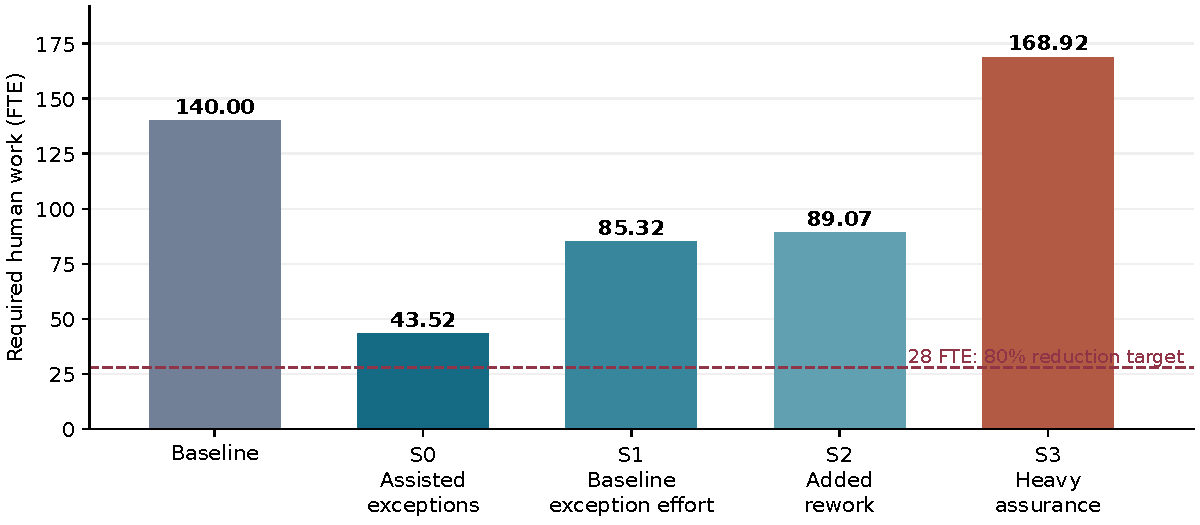
\includegraphics[width=0.88\linewidth]{figures/fig_labor_scenarios.pdf}
\caption{Illustrative human-work requirements with the same case partition: baseline 140 FTE;
four operating assumptions produce 43.52, 85.32, 89.07, and 168.92 FTE. The dashed line is the
author's 80\% reduction target, not a fitted forecast. Parameters and calculation are released.}
\label{fig:labor}
\end{figure}
These are sensitivity calculations using declared assumptions, not measurements or
forecasts. The comparison establishes a useful non-identification result: even fixed
coverage and a fixed baseline case partition do not determine the sign of the labor
effect. Their associated quality is not estimated. A deployment must measure both the
contract outcomes and the complete account to identify whether execution has actually
been substituted at acceptable quality.
None of these four scenarios reaches an 80\% reduction. With $\phi\simeq0.4686$ and no other
residual burden, that target already requires $\eta\le0.20/\phi\simeq0.427$.
Thus the forecast requires further reduction in exception effort or in its retained labor
share, even before allowing for ongoing review and support.

\paragraph{From required work to staffing.}
At fixed useful capacity $K>0$, required workload-equivalent FTE equal $L/K$. Under the
additional assumptions of interchangeable workers, target utilization $0<u\le1$, no separate
coverage constraint, and staffing chosen to minimize labor cost, required headcount is
$\lceil L/(uK)\rceil$. Reducing required hours then removes posts when this integer crosses
a staffing threshold. Redeployment or increased demand can absorb the released capacity;
they do not make execution of the old tasks indispensable again. For a finite collection
of gates with bounded visit counts, vanishing human case effort leaves a support floor
$B_A/K$; zero total human labor further requires that this support work be eliminated or
automated. These are explicit conditions for displacement, not a claim that current
benchmark performance has already satisfied them.

\section{From task substitution to a workforce hypothesis}
\label{sec:implications}

The observations support a positive, bounded conclusion: software can execute the specified
governance-review operations in this engineered environment. The deterministic control makes
the case for an executable decision kernel especially clear. The agents demonstrate another
implementation of many of these operations, with measurable differences in evidence handling,
reliability, and cost. Neither result is weakened by the fact that software uses several kinds
of components. What remains unresolved is the effort needed to construct and operate the
interfaces when facts and policies arrive in less prepared forms.

This is also where the claim about human replacement becomes testable. If a deployed system
performs accepted tasks previously executed by people and satisfies the labor inequality at
unchanged output and quality, it has substituted for part of their work. Calling the remaining
people supervisors does not restore the eliminated execution hours. At fixed demand, fewer
required hours can support fewer posts; actual headcount also depends on allocation, utilization,
redeployment, and new work. The argument therefore permits substantial workforce displacement
without treating it as a measured consequence of this synthetic experiment.

\subsection{The 2033 hypothesis and a falsifiable deployment test}

The author's original hypothesis is that the DGF ecosystem will require at least 80\% fewer
workload-equivalent FTE by 20 September 2033 than during the reference year ending on
20 September 2026, at comparable governed output, quality, and service. The boundary includes
preparation, exceptions, verification, remediation of review errors, maintenance, supervision,
and supplier support. On an illustrative 140-FTE baseline, the target is at most 28 FTE.
This is an author-selected forecast, not an extrapolation fitted to benchmark scores.

The baseline window has already closed and no enterprise cohort has been enrolled. Testing
this exact dated hypothesis requires auditable historical activity records and a declared
population and aggregation rule before observing its endpoint. Otherwise it cannot be scored
as confirmed. A newly registered baseline can support a separate seven-year prospective test,
but cannot move the date of the original prediction. A credible test fixes the accounting
boundary, useful-hours conversion, output mix, quality tolerances, and service levels. It
reports the complete $L_A/L_H$ account rather than headcount in a renamed department. A ratio
above 0.20 at the deadline fails the proposed 80\% target; achieving that ratio while degrading
the fixed quality or service requirements also fails the substitution claim. Missing records
make the result unassessable, not successful.

Full elimination of human DGF execution is a stronger, undated conjecture. It would require
both case-level human effort and the recurring support floor to disappear. No finite benchmark
here establishes that endpoint. The scientifically actionable question is how much accepted
task execution can already be transferred and what prevents further transfer.

\subsection{The next discriminating experiment}

The most useful extension varies information preparation while preserving answerability.
Compare agents receiving structured snapshots with agents receiving the source documents and
operational records from which the same facts can be recovered. Separately vary executable
versus natural-language policy. Fix source access, mandate, time and tool budgets, and the
evidence contract before testing on held-out cases. Include the rule engine and any required
extraction pipeline in the comparison. Report decision quality, supported findings, complete
routes, abstention, and all engineering and operating costs.

This extension does not require claiming human-level accuracy. It asks which parts of a review
the system can perform when the required facts are no longer supplied as a ready-to-use snapshot.
Our counterexample means that simply deleting snapshots is not a valid design. The released
source audit also identifies runtime tools that can return snapshots, so changing file visibility
alone would not isolate the intended condition. The existing extraction ablation and General-only
intervention are preparations, not additional measured results in this paper.

\subsection{Limits of the present evidence}

The benchmark's policy, generator, and reference share an author-designed rule system; their
agreement is internal consistency rather than validation of a universal business standard.
Decision-balanced synthetic cases do not estimate enterprise prevalence. There are three
endpoints, one original trajectory per model and case, and repetitions on only 15 existing
dossiers. The post-hoc structural evidence metric is not semantic adjudication. No measured
human comparator, enterprise deployment, staffing effect, or comparative ranking of candidate
business functions is available. These limits locate the evidence: execution of declared review
contracts is measured; net labor substitution and the 2033 forecast remain hypotheses to test.

\section{Conclusion}

The last human gate is not defined by the last person to hold an approval title. It is the last
task whose execution still requires human work after the evidence, policy, authority, and
supporting services have been specified. A governance function can remain mandatory while
software takes over tasks that previously required specialists to perform each review.

The DGF is a credible candidate for this transition because it already packages many of those
tasks into repeated, documented decision interfaces. Our contribution makes the substitution
claim conditional and measurable: sufficient accessible information, valid authorized outputs,
and a complete human-work account. The model explains why broad case coverage can coexist
with either a large reduction or an increase in required labor. The FDE implementation connects
these conditions to evidence services, policy checks, mandates, handoffs, and exception handling.

DGF-Bench demonstrates substantial execution capability for specified review tasks and exposes
the limits of inferring workflow reliability from correct decisions. Its deterministic control
also shows that a formalized review kernel can be executed without a language model. The
consequent research question is where agents can extend that kernel into less formalized work
at acceptable quality and lower total human effort. If they do so, replacement of human task
execution is the result, not merely an improvement in report drafting. Whether that reaches the
author's 80\% DGF-FTE reduction by 2033 requires the separate observations and fixed boundary
specified here.

\section*{Data, code, and attribution}

Jeremy Canale is the author: \texttt{contact@jeremycanale.com},
\url{https://www.jeremycanale.com}, \url{https://www.linkedin.com/in/jcanale13}.
The public repository is \url{https://github.com/jeremy1392/dgf-agentic-bench}.
Its \href{https://github.com/jeremy1392/dgf-agentic-bench/releases/tag/dgf-bench-300-20260923}{\texttt{dgf-bench-300-20260923}}
release contains the source snapshot, complete generated dossiers including Word documents and
architectures, model traces, failed attempts, scores, and cost ledgers. Original results and
offline reproduction are in \nolinkurl{research/2026-09-dgf-bench/}; controls, all-model evidence
audits, repetitions, and source counterexamples are in \nolinkurl{research/2026-09-followup/}.
Use the frozen experimental source to reproduce the collected run. Synthetic workforce
parameters are in \nolinkurl{paper/anc/parameters.json}; this concise manuscript and its
verification script are in \nolinkurl{paper2/}. The extended manuscript remains in
\nolinkurl{paper/}. Earlier empirical-companion versions remain in repository history.
No new model calls or human studies were conducted for this synthesis. The author is
responsible for the claims, artifacts, and interpretation.

% Checked primary-source metadata, 24 September 2026. Cite only entries used.
\begin{thebibliography}{99}
\raggedright

\bibitem[Acemoglu and Restrepo(2019)]{acemoglu2019}
Daron Acemoglu and Pascual Restrepo.
\newblock Automation and new tasks: How technology displaces and reinstates labor.
\newblock \emph{Journal of Economic Perspectives}, 33(2):3--30, 2019.
\newblock \url{https://doi.org/10.1257/jep.33.2.3}.

\bibitem[Bainbridge(1983)]{bainbridge1983}
Lisanne Bainbridge.
\newblock Ironies of automation.
\newblock \emph{Automatica}, 19(6):775--779, 1983.
\newblock \url{https://doi.org/10.1016/0005-1098(83)90046-8}.

\bibitem[Calvanese et~al.(2026)]{calvanese2026}
Diego Calvanese, Angelo Casciani, Giuseppe De~Giacomo, Marlon Dumas, Fabiana Fournier,
Timotheus Kampik, Emanuele La~Malfa, Lior Limonad, Andrea Marrella, Andreas Metzger,
Marco Montali, Daniel Amyot, Peter Fettke, Artem Polyvyanyy, Stefanie Rinderle-Ma,
Sebastian Sardi\~na, Niek Tax, and Barbara Weber.
\newblock Agentic business process management: A research manifesto.
\newblock \emph{Information Systems}, 140:102738, 2026.
\newblock \url{https://doi.org/10.1016/j.is.2026.102738}.

\bibitem[Cooper(1990)]{cooper1990}
Robert~G. Cooper.
\newblock Stage-gate systems: A new tool for managing new products.
\newblock \emph{Business Horizons}, 33(3):44--54, 1990.
\newblock \url{https://doi.org/10.1016/0007-6813(90)90040-I}.

\bibitem[Demirer et~al.(2026)]{demirer2026}
Mert Demirer, John~J. Horton, Nicole Immorlica, Brendan Lucier, and Peyman Shahidi.
\newblock Chaining tasks, redefining work: A theory of AI automation.
\newblock NBER Working Paper 34859, 2026.
\newblock \url{https://arxiv.org/abs/2606.15960}.

\bibitem[Drouin et~al.(2024)]{drouin2024}
Alexandre Drouin, Maxime Gasse, Massimo Caccia, Issam~H. Laradji, Manuel Del~Verme,
Tom Marty, David Vazquez, Nicolas Chapados, and Alexandre Lacoste.
\newblock WorkArena: How capable are web agents at solving common knowledge work tasks?
\newblock In \emph{Proceedings of the 41st International Conference on Machine Learning},
PMLR 235:11642--11662, 2024.
\newblock \url{https://proceedings.mlr.press/v235/drouin24a.html}.

\bibitem[Gans and Goldfarb(2026)]{gans2026}
Joshua~S. Gans and Avi Goldfarb.
\newblock O-Ring automation.
\newblock NBER Working Paper 34639, 2026.
\newblock \url{https://doi.org/10.3386/w34639}.

\bibitem[Gao et~al.(2023)]{gao2023}
Tianyu Gao, Howard Yen, Jiatong Yu, and Danqi Chen.
\newblock Enabling large language models to generate text with citations.
\newblock EMNLP, 2023.
\newblock \url{https://arxiv.org/abs/2305.14627}.

\bibitem[Jha et~al.(2025)]{itbench2025}
Saurabh Jha, Rohan Arora, Yuji Watanabe, Takumi Yanagawa, Yinfang Chen, et~al.
\newblock ITBench: Evaluating AI agents across diverse real-world IT automation tasks.
\newblock arXiv:2502.05352, 2025.
\newblock \url{https://arxiv.org/abs/2502.05352}.

\bibitem[Kapoor et~al.(2024)]{kapoor2024}
Sayash Kapoor, Benedikt Stroebl, Zachary~S. Siegel, Nitya Nadgir, and Arvind Narayanan.
\newblock AI agents that matter.
\newblock arXiv:2407.01502, 2024.
\newblock \url{https://arxiv.org/abs/2407.01502}.

\bibitem[Ly et~al.(2015)]{ly2015}
Linh Thao Ly, Fabrizio Maria Maggi, Marco Montali, Stefanie Rinderle-Ma,
and Wil M.~P. van~der Aalst.
\newblock Compliance monitoring in business processes: Functionalities, application, and tool-support.
\newblock \emph{Information Systems}, 54:209--234, 2015.
\newblock \url{https://doi.org/10.1016/j.is.2015.02.007}.

\bibitem[Palantir Technologies(2026)]{palantirfde2026}
Palantir Technologies.
\newblock Forward Deployed Software Engineer.
\newblock Official role description, accessed 24 September 2026.
\newblock \url{https://jobs.lever.co/palantir/dab396d4-2f14-4796-aac0-0d82883dccf0}.

\bibitem[Rashkin et~al.(2023)]{rashkin2023}
Hannah Rashkin, Vitaly Nikolaev, Matthew Lamm, Lora Aroyo, Michael Collins,
Dipanjan Das, Slav Petrov, Gaurav Singh Tomar, Iulia Turc, and David Reitter.
\newblock Measuring attribution in natural language generation models.
\newblock \emph{Computational Linguistics}, 49(4):777--840, 2023.
\newblock \url{https://aclanthology.org/2023.cl-4.2/}.

\bibitem[Yao et~al.(2024)]{taubench2024}
Shunyu Yao, Noah Shinn, Pedram Razavi, and Karthik Narasimhan.
\newblock $\tau$-bench: A benchmark for tool-agent-user interaction in real-world domains.
\newblock arXiv:2406.12045, 2024.
\newblock \url{https://arxiv.org/abs/2406.12045}.

\end{thebibliography}

\appendix
\section{Complete decision confusion matrices}

Rows use the effective reference after validated authority actions; columns are the model's
submitted disposition. G = GO, C = GO\_WITH\_RESERVATIONS, R = REWORK, S = SUSPENSION,
N = NO\_GO. All original evaluable gates are included. The released summary also permits comparison
with the separately reported initial-reference agreement.

\begingroup
\captionsetup{hypcap=false}
\begin{center}
\small
\captionof{table}{DeepSeek disposition confusion; 1700 evaluable gates.}
\begin{tabular}{@{}lrrrrr@{}}
\toprule
Reference / predicted & G & C & R & S & N\\
\midrule
G & 441 & 3 & 35 & 9 & 0\\
C & 0 & 302 & 23 & 1 & 0\\
R & 0 & 0 & 416 & 2 & 1\\
S & 0 & 0 & 3 & 186 & 2\\
N & 1 & 0 & 1 & 0 & 274\\
\bottomrule
\end{tabular}
\end{center}

\begin{center}
\small
\captionof{table}{Gemini disposition confusion; 1694 evaluable gates.}
\begin{tabular}{@{}lrrrrr@{}}
\toprule
Reference / predicted & G & C & R & S & N\\
\midrule
G & 488 & 0 & 0 & 0 & 0\\
C & 0 & 398 & 0 & 0 & 0\\
R & 0 & 0 & 352 & 0 & 0\\
S & 0 & 0 & 0 & 180 & 0\\
N & 0 & 0 & 0 & 0 & 276\\
\bottomrule
\end{tabular}
\end{center}

\begin{center}
\small
\captionof{table}{Luna disposition confusion; 1700 evaluable gates.}
\begin{tabular}{@{}lrrrrr@{}}
\toprule
Reference / predicted & G & C & R & S & N\\
\midrule
G & 482 & 4 & 3 & 0 & 0\\
C & 0 & 354 & 3 & 0 & 0\\
R & 1 & 0 & 394 & 0 & 0\\
S & 0 & 0 & 17 & 166 & 0\\
N & 0 & 0 & 3 & 1 & 272\\
\bottomrule
\end{tabular}
\end{center}

\endgroup


\section{Reproduction record}

The public research package contains the complete original and repeated-run traces, unchanged
primary scores, per-item all-model evidence classifications, strict and post-hoc route outcomes,
confusion matrices, and counterfactual document hashes. Analysis scripts use the frozen benchmark
source archive. They make no inference calls and do not overwrite original scores. The manuscript
verification script checks published counts and the provenance of inherited tables and figures.
These checks establish reproducibility and internal consistency; they do not provide independent
professional validation of the rule system.

\end{document}
